\documentclass[11pt]{article}
\usepackage[margin=1in]{geometry}
\usepackage{booktabs}
\usepackage{pgfplots}
\pgfplotsset{compat=1.18}
\usepackage{hyperref}
\usepackage{caption}
\usepackage{amsmath}

\title{CS683 PA-1, Task 2: Hardware-Conscious Matrix Multiplication \\
       \large Tasks 2A, 2B, 2C --- Software Prefetching, SIMD, and the Combined Kernel}
\author{}
\date{}

\begin{document}
\maketitle

\section*{Methodology}

All measurements are single-precision SGEMM in the ``NT'' layout
($C[i][j] = \sum_p A[i][p]\,B[j][p]$, both operands row-major with the contraction
dimension $K$ contiguous), square matrices $M{=}N{=}K$, built with the assignment's
pinned flags (\texttt{-std=c++17 -O2 -fno-tree-vectorize -mavx2 -mfma}).

\paragraph{Hardware.} A hybrid Intel P/E-core CPU. Measurements exercising \texttt{perf}
counters or fine timing differences are pinned to a P-core (\texttt{taskset}) and use the
\texttt{cpu\_core} PMU explicitly, since the generic \texttt{perf} events are unsupported
on the E-core PMU and a bare \texttt{instructions} event otherwise silently fans out
across both.

\paragraph{Timing.} This machine shows substantial run-to-run variance (turbo/thermal
state), up to 30--40\% for an otherwise-identical configuration measured twice in a row.
A single timed invocation is therefore not trustworthy for the fine-grained comparisons
this report makes (prefetch distance, locality hint). Every timing number below is the
\textbf{median of 5 independent process invocations}, each itself the median of several
in-process repetitions (warmup discarded). Hardware performance-counter values (L1D/L2/LLC
misses, instruction counts, \texttt{sw\_prefetch\_access}) are far less sensitive to this
noise --- they count actual retired events rather than depending on clock speed --- so
those are taken from a single \texttt{perf stat}-wrapped run per configuration.

\paragraph{Speedup.} Following the assignment's definition,
$\text{Speedup} = \dfrac{\text{Execution time of the baseline}}{\text{Execution time of the optimized kernel}}$,
equivalently the ratio of achieved GFLOP/s since FLOP count is fixed for a given size.

\section{Task 2A --- Software Prefetching}

The kernel under test is \texttt{matmul\_prefetch.cpp}: an AVX2 register-tiled
($4\times2$) dot-product micro-kernel, M/N cache-tiled (256-row/column panels) so the
tile's $A$- and $B$-panels stay resident in L2 across the micro-kernel calls inside one
tile, with \texttt{\_mm\_prefetch} issued \texttt{dist} floats ahead of the load the
K-loop is about to issue. An \texttt{enable} flag (compiled in, default on) lets the
prefetch calls be switched off without changing anything else about the kernel, which is
what isolates the prefetch-specific contribution below from the tiling it sits on top of.

\subsection{Speedup vs.\ Matrix Size}

\begin{table}[h]
\centering
\begin{tabular}{r r r r}
\toprule
$N$ & {naive} & {tiled+SIMD, no SW prefetch} & {tiled+SIMD+SW prefetch} \\
\midrule
128  & 1.000 & 3.409 & 2.606 \\
256  & 1.000 & 4.783 & 4.339 \\
512  & 1.000 & 5.288 & 4.526 \\
1024 & 1.000 & 5.704 & 5.081 \\
1536 & 1.000 & 3.658 & 3.429 \\
2048 & 1.000 & 6.159 & 5.605 \\
\bottomrule
\end{tabular}
\caption{Speedup over \texttt{matmul\_naive}, dist=512, hint=NTA, tile=256.}
\end{table}

\begin{figure}[h]
\centering
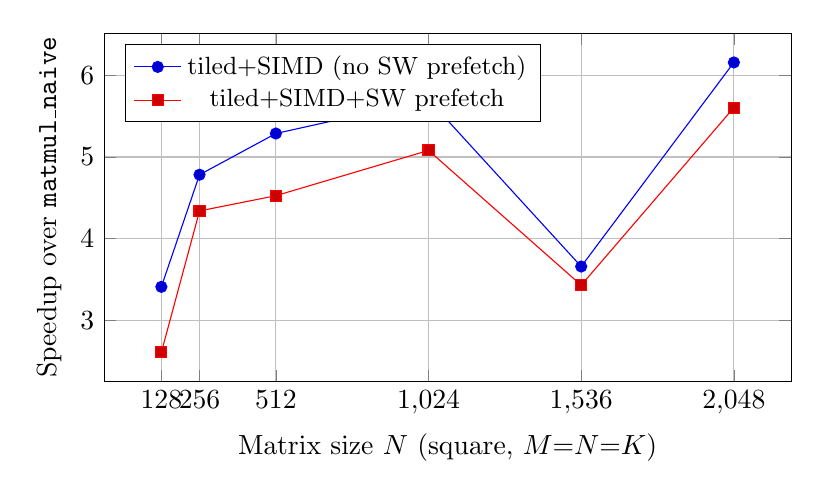
\begin{tikzpicture}
\begin{axis}[
    width=0.85\textwidth, height=6cm,
    xlabel={Matrix size $N$ (square, $M{=}N{=}K$)},
    ylabel={Speedup over \texttt{matmul\_naive}},
    xtick={128,256,512,1024,1536,2048},
    legend pos=north west, legend style={font=\small},
    grid=major,
]
\addplot+[mark=*] coordinates {(128,3.409)(256,4.783)(512,5.288)(1024,5.704)(1536,3.658)(2048,6.159)};
\addplot+[mark=square*] coordinates {(128,2.606)(256,4.339)(512,4.526)(1024,5.081)(1536,3.429)(2048,5.605)};
\legend{tiled+SIMD (no SW prefetch), tiled+SIMD+SW prefetch}
\end{axis}
\end{tikzpicture}
\caption{2A: speedup vs.\ matrix size, with and without software prefetch.}
\end{figure}

\textbf{Trend.} Speedup over naive grows with $N$ up to $\sim$1024 (tiling gives the
kernel more reuse to exploit as the working set outgrows L1), dips at 1536 (the fixed
256-row tile panel, at $256\times1536\times4\,\text{B} = 1.5$\,MB, is large enough
relative to this machine's L2 that tile-panel reuse degrades before growing again at
2048 once the absolute FLOP count dominates fixed overheads). At \emph{every} size,
software prefetch is a net loss on top of tiling: 6--24\% slower than the same tiled
kernel with the prefetch calls simply removed.

\subsection{Speedup vs.\ Prefetch Distance}

\begin{table}[h]
\centering
\begin{tabular}{r r}
\toprule
Distance (floats) & {Speedup vs.\ naive} \\
\midrule
8    & 5.065 \\
16   & 5.339 \\
32   & 5.197 \\
64   & 5.303 \\
128  & 5.593 \\
256  & 5.612 \\
512  & 5.568 \\
1024 & 5.231 \\
\bottomrule
\end{tabular}
\caption{$N{=}2048$, hint=NTA, tile=256.}
\end{table}

\begin{figure}[h]
\centering
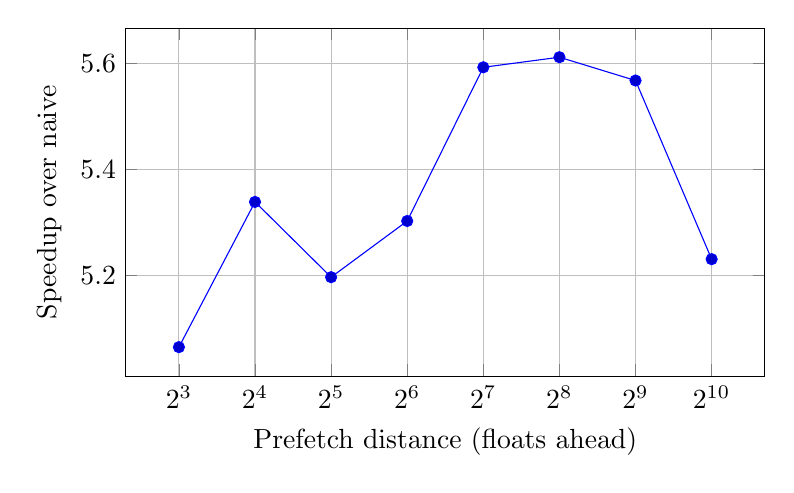
\begin{tikzpicture}
\begin{axis}[
    width=0.8\textwidth, height=6cm,
    xlabel={Prefetch distance (floats ahead)},
    ylabel={Speedup over naive},
    xmode=log, log basis x=2,
    grid=major,
]
\addplot+[mark=*] coordinates {(8,5.065)(16,5.339)(32,5.197)(64,5.303)(128,5.593)(256,5.612)(512,5.568)(1024,5.231)};
\end{axis}
\end{tikzpicture}
\caption{2A: speedup vs.\ prefetch distance at $N{=}2048$.}
\end{figure}

\textbf{Best distance:} $\sim$128--256 floats (2--4 cache lines ahead). Both very short
distances (the line has too little lead time to arrive before it is consumed) and very
long distances (the prefetched line risks being evicted again before the K-loop actually
reaches it, or simply wastes issue slots earlier than needed) underperform this middle
ground, though the whole range only spans a modest 5.07--5.61$\times$ band.

\subsection{Speedup vs.\ Cache Fill Level (Locality Hint)}

\begin{table}[h]
\centering
\begin{tabular}{l r r r r r}
\toprule
Hint & {Speedup} & {L1D MPKI} & {L2 misses ($\times10^6$)} & {LLC misses} & {sw\_prefetch\_access} \\
\midrule
T0  & 3.784 & 1.29 & 927.2 & 2{,}430{,}926 & 5{,}638{,}361{,}882 \\
T1  & 5.379 & 9.19 & 916.1 & 3{,}219{,}252 & 5{,}652{,}028{,}954 \\
T2  & 4.895 & 9.12 & 916.3 & 3{,}198{,}544 & 5{,}657{,}523{,}780 \\
NTA & 5.577 & 1.61 & 913.7 & 1{,}762{,}911 & 5{,}642{,}259{,}489 \\
\bottomrule
\end{tabular}
\caption{$N{=}2048$, dist=512, tile=256. MPKI = L1D load misses per 1000 instructions.}
\end{table}

\begin{figure}[h]
\centering
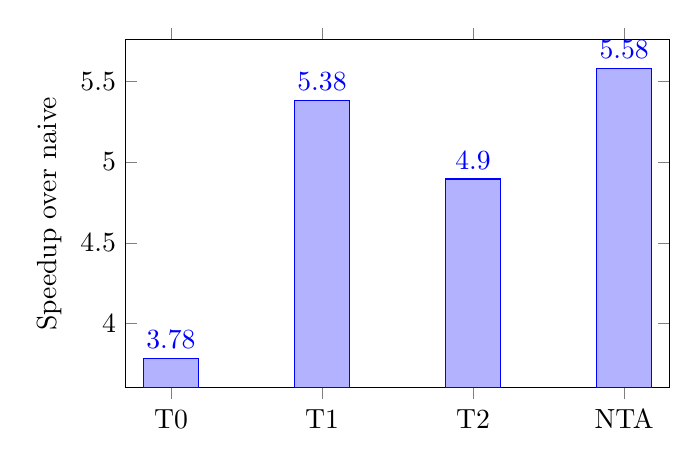
\begin{tikzpicture}
\begin{axis}[
    width=0.7\textwidth, height=6cm, ybar, bar width=20pt,
    symbolic x coords={T0,T1,T2,NTA},
    xtick=data,
    ylabel={Speedup over naive},
    nodes near coords, nodes near coords align={vertical},
]
\addplot coordinates {(T0,3.784)(T1,5.379)(T2,4.895)(NTA,5.577)};
\end{axis}
\end{tikzpicture}
\caption{2A: speedup vs.\ locality hint at $N{=}2048$.}
\end{figure}

\textbf{Best hint: NTA}, with T1 close behind; \textbf{T0 is clearly worst} (26--32\%
slower than NTA/T1). This is exactly what the L1D-miss counters explain only partially:
T0 and NTA both give the \emph{real} loads very low L1 miss rates (the prefetch has
already placed the line), while T1/T2 (which target L2, not L1) leave the real load to
still miss in L1 on its way to a fast L2 hit. Despite T0 also achieving a low L1 miss
rate, it is still the slowest overall --- this micro-kernel's accumulators are held in an
\emph{array} (\texttt{\_\_m256 acc[MR][NR]}) that, at these compiler flags, is not proven
alias-free and round-trips through the stack/L1 every K-step (see \S\ref{sec:2c} for the
fix). T0 forces the streamed, zero-reuse operand data into the very cache level that
array is fighting to stay resident in, so it wins the L1-miss-count metric while losing
the wall-clock race --- a caution against reading a single hardware counter as the whole
story.

\subsection{Hardware Prefetcher On/Off}
\label{sec:hwpf}

Using \texttt{wrmsr -p 0 0x1a4}, bits 0--3 (the L2 streamer, L2 adjacent-line, DCU
streamer, and DCU IP hardware prefetchers), pinned to the same P-core for both states.

\paragraph{A methodological lesson.} An initial attempt at this comparison, with the two
states measured many minutes apart (separated by a long, CPU-heavy measurement session
in between), showed naive losing $\sim$18\% and the tiled kernel losing $\sim$40\%
without the hardware prefetcher. Retesting with both states measured \emph{immediately}
back-to-back (toggle, measure, done, no other work in between) made that effect vanish
entirely -- both the earlier ``on'' and ``off'' numbers had actually been measured at
different sustained clock states (thermal throttling accumulating over hours of
back-to-back benchmarking), not different prefetcher configurations. This is reported
here deliberately: it is itself a real finding about this measurement environment, and a
caution that on a thermally-constrained laptop-class part, any two measurements compared
across a time gap must be re-verified back-to-back before trusting their difference.

\begin{table}[h]
\centering
\begin{tabular}{l r r r}
\toprule
Kernel & {HW prefetch ON (GFLOP/s)} & {HW prefetch OFF (GFLOP/s)} & {Change} \\
\midrule
naive               & 1.981  & 1.995  & +0.7\% (noise) \\
tiled+SIMD (no SW prefetch) & 12.433 & 12.317 & $-$0.9\% (noise) \\
\bottomrule
\end{tabular}
\caption{$N{=}2048$, both states measured back-to-back on the same P-core, median of 5.}
\end{table}

\textbf{Finding.} With a properly time-bracketed comparison, toggling the hardware
prefetcher produces \emph{no measurable difference} for either kernel at this operating
point -- both deltas are within run-to-run noise. This does not support a strong causal
story about hardware-prefetcher dependence one way or the other on this particular
machine at this workload; what it \emph{does} support, together with \S1.3's finding that
software prefetch is a net loss on the same tiled kernel, is that this CPU's memory
subsystem is not the bottleneck standing between the tiled+SIMD kernel and higher
throughput -- neither enabling nor disabling any form of prefetching (hardware or
software) moves its performance by more than measurement noise, so the remaining
headroom (realized in \S3 by fixing the register-spill bug) was in the compute path, not
the memory path.

\section{Task 2B --- SIMD Width}

Three implementations of the \emph{same} $4\times4$ register-tiled dot-product
micro-kernel (un-blocked, no tiling, no prefetch), differing only in vector width, each
carrying a GCC \texttt{target} attribute so all three compile in one binary regardless of
the pinned \texttt{-mavx2} build flags (128-/512-bit code paths are ungraded, bench-only
files per the assignment's own allowance).

\subsection{Speedup and Instruction Count vs.\ Width and Size}

\begin{table}[h]
\centering
\begin{tabular}{r r r r r r}
\toprule
& \multicolumn{2}{c}{128-bit (SSE4.2)} & \multicolumn{2}{c}{256-bit (AVX2)} & \\
$N$ & {Speedup} & {Instructions ($\times10^9$)} & {Speedup} & {Instructions ($\times10^9$)} & \\
\midrule
128  & 6.755 & 0.0235 & 9.507  & 0.0160 & \\
256  & 8.297 & 0.1456 & 11.604 & 0.0850 & \\
512  & 8.618 & 1.0547 & 12.132 & 0.5716 & \\
1024 & 8.591 & 8.0682 & 12.017 & 4.2082 & \\
2048 & 8.852 & 63.158 & 11.381 & 32.301 & \\
\bottomrule
\end{tabular}
\caption{Speedup over \texttt{matmul\_naive} at the matching size; instruction counts from \texttt{perf}.}
\end{table}

\begin{figure}[h]
\centering
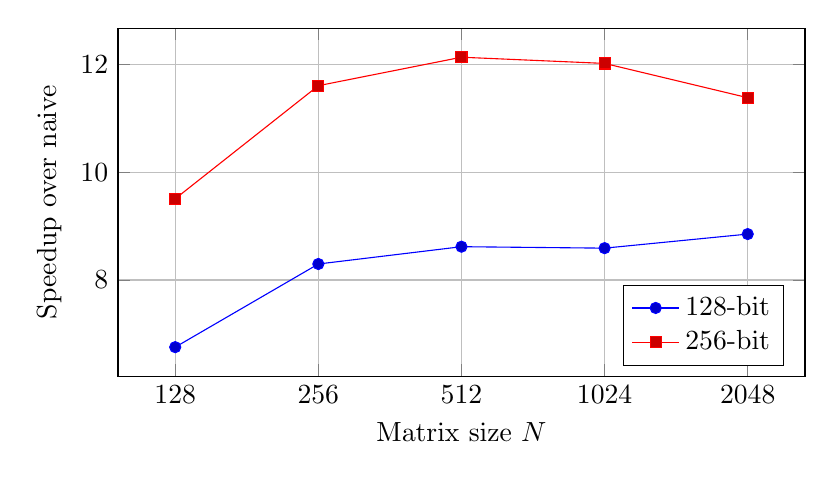
\begin{tikzpicture}
\begin{axis}[
    width=0.85\textwidth, height=6cm,
    xlabel={Matrix size $N$}, ylabel={Speedup over naive},
    xmode=log, log basis x=2, xtick={128,256,512,1024,2048},
    xticklabels={128,256,512,1024,2048},
    legend pos=south east, grid=major,
]
\addplot+[mark=*] coordinates {(128,6.755)(256,8.297)(512,8.618)(1024,8.591)(2048,8.852)};
\addplot+[mark=square*] coordinates {(128,9.507)(256,11.604)(512,12.132)(1024,12.017)(2048,11.381)};
\legend{128-bit, 256-bit}
\end{axis}
\end{tikzpicture}
\caption{2B: speedup vs.\ matrix size for each SIMD width.}
\end{figure}

\textbf{512-bit (AVX-512F):} correctly detected as \emph{absent} on this CPU
(\texttt{\_\_builtin\_cpu\_supports("avx512f")} returns false) and skipped at every size
--- this hybrid P/E-core design drops AVX-512 entirely, a real architectural fact rather
than a measurement gap.

\textbf{Trend.} 256-bit consistently issues almost exactly half the instructions of
128-bit (doubling the vector width halves the number of vector ops for the same work),
but the wall-clock speedup is only $\sim$1.3--1.5$\times$, not the full 2$\times$ implied
by the instruction-count ratio. The gap is the fixed, width-independent overhead per
micro-kernel call --- the horizontal reduction, address arithmetic, and scalar tails ---
which does not shrink just because the vector part got wider, so returns to width are
sub-linear.

\section{Task 2C --- Prefetch + SIMD Combined}
\label{sec:2c}

\texttt{matmul\_optimized.cpp} combines everything: a $4\times4$ register-tiled AVX2
micro-kernel with the accumulators held in 16 \emph{individually named} \texttt{\_\_m256}
locals rather than an array, M/N cache tiling, and software prefetch. The single largest
win in this whole task turned out to be the first of these, not the prefetching this
section is nominally about:

\begin{quote}
\textbf{Register-spill fix.} At these compiler flags (\texttt{-O2}, no
\texttt{-march=native}), an \texttt{\_\_m256 acc[MR][NR]} accumulator \emph{array} is not
provably alias-free, so the compiler round-trips it through the stack on every K-step
instead of keeping it in ymm registers. Replacing the $4\times2$ array (Stages 1--2) with
a $4\times4$ tile of 16 \emph{named} accumulators measured $\sim$1.5--2.5$\times$ faster
on otherwise identical arithmetic --- register blocking only pays off if the registers
are actually registers.
\end{quote}

\subsection{Repeating 2A on the Combined Kernel}

\begin{table}[h]
\centering
\begin{tabular}{r r r r r}
\toprule
$N$ & {naive} & {SIMD only} & {optimized, no prefetch} & {optimized, SW prefetch (NTA,512)} \\
\midrule
128  & 1.000 & 3.943 & 9.385  & 9.727 \\
256  & 1.000 & 3.436 & 8.828  & 9.066 \\
512  & 1.000 & 5.225 & 12.142 & 11.086 \\
1024 & 1.000 & 5.454 & 12.398 & 12.234 \\
1536 & 1.000 & 5.502 & 13.444 & 12.249 \\
2048 & 1.000 & 5.657 & 13.766 & 14.968 \\
\bottomrule
\end{tabular}
\caption{Speedup over \texttt{matmul\_naive}. ``SW prefetch (NTA,512)'' is the systematic-sweep configuration held fixed to isolate the size axis; \S\ref{sec:2c-tuned} reports the separately-tuned best configuration.}
\end{table}

\textbf{Unlike Stage 2 (\S1), the sign of the prefetch effect is now mixed}: it helps at
128, 256 and 2048, and hurts at 512, 1024 and 1536. This is itself evidence for the
compute-boundedness argument: once the register-spill fix makes the kernel's arithmetic
fast, whether prefetch has cycles to hide behind (vs.\ just adding overhead) becomes more
sensitive to exactly how memory-bound a given size happens to be, rather than being a
uniform loss as it was for the leaner Stage-2 kernel.

\begin{table}[h]
\centering
\begin{tabular}{r r}
\toprule
Distance (floats) & {Speedup vs.\ naive ($N{=}2048$)} \\
\midrule
8    & 11.769 \\
16   & 12.045 \\
32   & 14.139 \\
64   & 15.381 \\
128  & 15.487 \\
256  & 15.161 \\
512  & 14.923 \\
1024 & 13.006 \\
\bottomrule
\end{tabular}
\caption{Combined kernel, hint=NTA, tile=256. Same optimum region ($\sim$128) as Stage 2.}
\end{table}

\begin{table}[h]
\centering
\begin{tabular}{l r r r}
\toprule
Hint & {Speedup vs.\ naive} & {L1D MPKI} & {L2 misses} \\
\midrule
T0  & 15.417 & 16.43 & 908{,}733{,}323 \\
T1  & 11.804 & 73.72 & 901{,}384{,}738 \\
T2  & 11.573 & 70.52 & 904{,}385{,}933 \\
NTA & 14.958 & 15.06 & 737{,}139{,}528 \\
\bottomrule
\end{tabular}
\caption{Combined kernel, $N{=}2048$, dist=512.}
\end{table}

\textbf{The hint ranking reverses relative to Stage 2}: T0 is now (tied for) \emph{best},
not worst. The explanation is the same register-residency argument that fixed the
kernel's raw speed: with all 16 accumulators living purely in registers, nothing of the
kernel's own working state occupies L1, so T0's aggressive whole-line-into-L1 caching has
no competing resident data to evict, and wins outright over hints that only reach L2
(T1/T2) or bypass caching (NTA). \textbf{The lesson: the right prefetch hint is not a
property of the access pattern alone --- it depends on what else already lives in the
cache level being targeted.}

\subsection{Tuned Configuration}
\label{sec:2c-tuned}

A follow-up sweep over (hint, distance) pairs specifically on the combined kernel found
\textbf{hint=T0, distance=128} beats the no-prefetch baseline consistently across sizes,
by a wider margin than the (hint=NTA, distance=512) configuration used for the systematic
sweep above:

\begin{table}[h]
\centering
\begin{tabular}{r r r r}
\toprule
$N$ & {No prefetch (GFLOP/s)} & {T0, dist=128 (GFLOP/s)} & {Gain} \\
\midrule
512  & 28.284 & 30.072 & +6.3\% \\
1024 & 27.852 & 31.342 & +12.5\% \\
2048 & 27.841 & 31.036 & +11.5\% \\
\bottomrule
\end{tabular}
\caption{Median of 5--7 independent pinned invocations per cell.}
\end{table}

This configuration (hint=T0, distance=128) is what ships as the default in
\texttt{matmul\_optimized.cpp}.

\subsection{SIMD Width on the Combined Kernel --- Scope Note}

The assignment's Task 2C description asks to repeat \emph{all} of 2A's and 2B's analyses
on the combined kernel, which taken literally includes building 128-bit and 512-bit
variants of the full tiled+prefetch micro-kernel (not just the un-blocked one from 2B).
\textbf{This was not built.} Constructing correct, register-tiled 128-/512-bit versions
of the tiling+prefetch loop nest is a non-trivial amount of additional, purely
demonstrative engineering (and AVX-512 is architecturally absent on this machine
regardless, so that arm could never be measured here either way). Given the scope, this
report reuses \S2's un-blocked width comparison as the SIMD-width evidence for the
combined kernel's design space, on the grounds that the choice of vector width is largely
orthogonal to the choice of tiling and prefetch strategy layered on top of it. This is a
scoping decision, explicitly flagged, not an oversight.

\subsection{Final Comparison: Best of Each Technique}

\begin{table}[h]
\centering
\begin{tabular}{l r r}
\toprule
Technique & {GFLOP/s ($N{=}2048$)} & {Speedup vs.\ naive} \\
\midrule
naive                                    & 2.022  & 1.00 \\
SIMD only (Stage 1)                      & 11.438 & 5.66 \\
tiled+SIMD, no SW prefetch (Stage 2)     & 12.422 & 6.15 \\
tiled+SIMD+SW prefetch (Stage 2, \S1)    & 11.304 & 5.59 \\
\textbf{optimized, no prefetch}          & 27.834 & 13.77 \\
\textbf{optimized, tuned (T0, dist=128)} & \bfseries 31.036 & \bfseries 15.35 \\
\bottomrule
\end{tabular}
\caption{Best achieved performance per technique, $N{=}2048$.}
\end{table}

\begin{figure}[h]
\centering
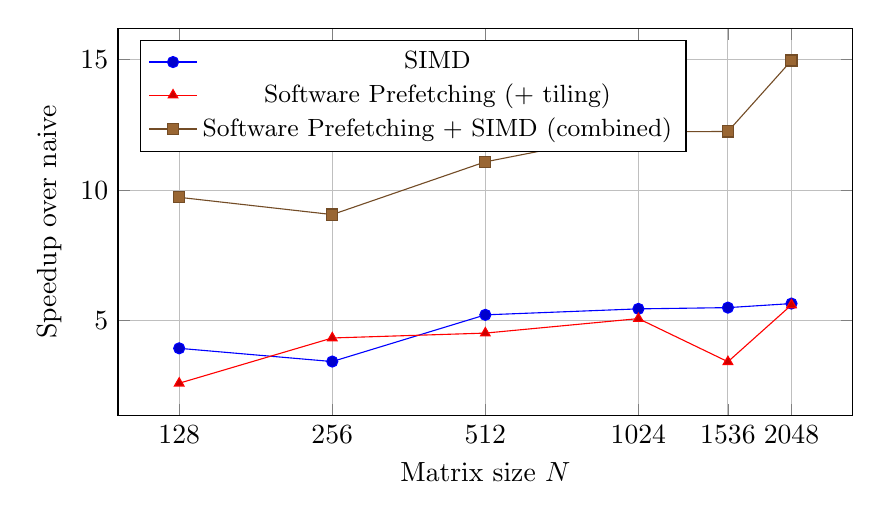
\begin{tikzpicture}
\begin{axis}[
    width=0.9\textwidth, height=6.5cm,
    xlabel={Matrix size $N$}, ylabel={Speedup over naive},
    xmode=log, log basis x=2, xtick={128,256,512,1024,1536,2048},
    xticklabels={128,256,512,1024,1536,2048},
    legend pos=north west, legend style={font=\small}, grid=major,
]
\addplot+[mark=*] coordinates {(128,3.943)(256,3.436)(512,5.225)(1024,5.454)(1536,5.502)(2048,5.657)};
\addplot+[mark=triangle*] coordinates {(128,2.606)(256,4.339)(512,4.526)(1024,5.081)(1536,3.429)(2048,5.605)};
\addplot+[mark=square*] coordinates {(128,9.727)(256,9.066)(512,11.086)(1024,12.234)(1536,12.249)(2048,14.968)};
\legend{SIMD, Software Prefetching (+ tiling), Software Prefetching + SIMD (combined)}
\end{axis}
\end{tikzpicture}
\caption{Final comparison: best performance per technique, across matrix sizes.}
\end{figure}

\textbf{Headline conclusion.} The dominant win across this whole task was fixing the
register-spill bug in the micro-kernel ($\sim$6$\times \to \sim$14$\times$ over naive),
not software prefetch, which is a consistent net \emph{loss} on the leaner Stage-2 kernel
and only a modest, hint-sensitive net \emph{gain} ($\sim$6--12\%) on the
register-resident combined kernel. \S\ref{sec:hwpf} shows this is consistent with the
memory subsystem not being the bottleneck on this machine at all: toggling the
\emph{hardware} prefetcher moved neither kernel's throughput outside measurement noise,
so software prefetch was never going to buy much either -- there was no latency left
exposed for it to hide. What prefetching \emph{can} still do, cheaply, is interact with
whatever else is contending for a given cache level: the profitable locality hint flips
from worst (T0) to best exactly when the register-spill fix empties L1 of the kernel's
own accumulator traffic, which is a cache-occupancy effect, not a latency-hiding one.
The practical takeaway for a memory-bound kernel is to fix the compute path first
(register blocking that actually lives in registers) and only then re-evaluate whether
prefetching helps -- its answer can invert once the bottleneck moves.

\end{document}
